% Feature - feature correlation before / after processing (correlation_heatmaps.py).
% Requires \usepackage{graphicx}. Two-column wide (figure*), at the top of the next page.
\begin{figure*}[t]
  \centering
  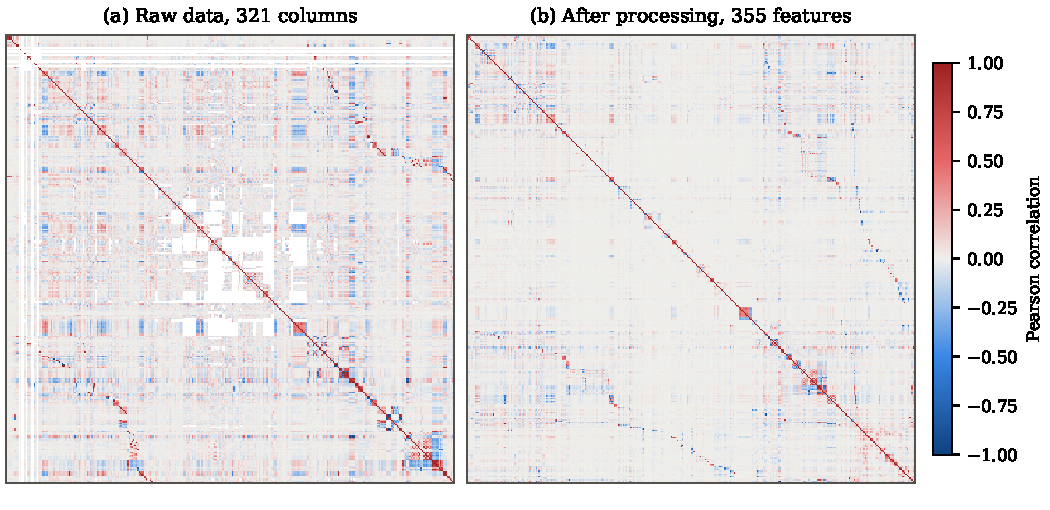
\includegraphics[width=\textwidth]{correlation_heatmaps.pdf}
  \caption{Feature--feature Pearson correlation. (a) Raw columns in survey order,
    once the ``don't know'' / ``refused'' codes are NaN; correlations use the rows
    where both columns are answered, white pairs share fewer than 100 such rows.
    (b) The features of the model after all processing steps: kept columns in survey
    order, each nominal column replaced by its dummies, then the missing indicators.}
  \label{fig:correlation}
\end{figure*}
